\chapter{Implementation, Analysis and Results}
{\color{red} 
	Investigating constraints impact in time windows was performed by analysing two different association networks; FSS-n and FBS-n.
	
	Those two different types of networks were applied in all ten time-window, and average modularity metric plots were generated. 
}

\section{Real-life Events}
\subsection*{Data Collection and Cleaning}
\addcontentsline{toc}{subsection}{Data Collection and Cleaning}%

The queries in Structured Query Language (SQL) were generated to find and pull the production orders data from the database across $2$--$3$ years of production work completed in the production lines, {\color{red}introduced in Table~\ref{Tab: production_lines}}. The SQL queries are given in the Supplementary Materials: \ref{figure-supplements-CCM_CSP-SQL}, \ref{figure-supplements-PLTCM-SQL}, and \ref{figure-supplements-CGL-SQL}.

At the beginning of the data cleaning process, the raw data was handled considering the string-type data values conversion into floating-point numbers, modifying inconsistent punctuation marks between digits into one typical style, and converting null values into the integer value $0$. 

After going over minor revision steps, we introduce some preconditions below to consider usable parts and fill the gaps in the data sets.
\begin{itemize}
	\item The steel material density was considered between $6.5 x 10^{-6}$ $kg/mm^{3}$ and $8.5 x 10^{-6}$ $kg/mm^{3}$. The production orders with density values out of that range were discarded from consideration.
	\item The production feature, length values were taken into account with millimetre (mm) units in the metric system.
	\item Machines input capacity limit ranges were identified for the production features; width, thickness, and weight as $800$--$2000$ mm, $40$--$90$ mm, and $2669$--$26690$ kg.
\end{itemize}

Considering the preconditions mentioned above and $density = mass/volume$ equality, $0$ values were replaced with the calculated values in every production order with a maximum of one unknown value from the features; width, thickness, weight, and length. {\color{red}Production orders (the so-called events)} with two missing values were compared with consecutive events, and missing terms were filled based on the consistency among the same sequence events. Sequences with less than $50$ events were removed from the data sets considering those short sequences might be generated for some test processes. At the final stage, obtained data set lengths are given below.
\begin{itemize}
	\item CCM data set: $347,418$ events.
	\item CSP data set: $205,496$ events.
	\item PLTCM data set: $64,026$ events.
	\item CGL data set: $31,230$ events.
\end{itemize}
The decreasing number of events through the data sets shows that the output of a production line is not always an input for the next in line and might be excluded from the continuous production line, as mentioned in {\color{red}the first section of the Introduction}.

\subsection*{Analysis Steps and Results}
\addcontentsline{toc}{subsection}{Analysis Steps and Results}%

The complete analysis of real-life events comprises a check for meaningful modularity structures in various dimensions for the association networks generated from the data collection. We introduce those dimensions as;
\begin{itemize}
	\item[1.] production line,
	\item[2.] production feature,
	\item[3.] production constraint,
	\item[4.] null model,
	\item[5.] time resolution, and
	\item[6.] network resolution.
\end{itemize} 
For the first dimension, distinguished data sets belonging to CCM, CSP, PLTCM, and CGL were considered in the given order considering {\color{red}the production portfolio evolves from producing products in a diverse range to producing specialised products from CCM to CGL}. The following dimensions were examined independently in each production line.

Since width and thickness are the products' physical quantities that are deliberately reformed during the whole manufacturing process, those data feature columns are taken into account for each production line to be analysed as the second dimension. 

{\color{red}Two fundamentally different constraints: technology-driven constraints and load-driven constraints are acting on the manufacturing process. Alternative binning methods and different network approaches were identified for those constraints. FSS and FBS networks were generated in the third dimension for each production feature in every production line.}

NM-d and NM-m, as previously introduced, were considered to check the randomness of the association networks. As the fourth dimension, those alternative null models were constructed for each FSS and FBS network generated. Resulted z-scores are more straightforward than the resulted modularity values since they take out any effect from different link densities. For this reason, we shared only z-scores as bar charts in this subsection and attached the bar charts and curve plots for the modularity values as supplementary materials.

Time resolution is the fifth dimension, and it consists of different observation-window categories as discrete-time windows, sliding-time windows and complete data with two halves. Each resolution is a means of partitioning the data of historically ordered production events into equal sizes differently. For each window in three categories, the first four dimensions were performed. The analysis with time-resolved fashion allows checking if any significant constraint impact reveals systematically through the time windows created with varying sizes. Since the most significant results were obtained from the last category, the complete data with two halves, we shared and discussed that category in this subsection. The analysis results for discrete-time windows and sliding-time windows are supplementary materials: \ref{figure-supplements-CCM_CSP-curveplots_discrete}, \ref{figure-supplements-PLTCM_CGL-curveplots_discrete} and \ref{figure-supplements-CCM-curveplots_sliding}, \ref{figure-supplements-CSP-curveplots_sliding}, \ref{figure-supplements-PLTCM-curveplots_sliding}, \ref{figure-supplements-CGL-curveplots_sliding}.

As the last dimension, association networks obtained from the first four dimensions in the observation-window categories: the sliding-time windows and the complete data with two halves, were diversified in two different network resolutions by changing the node amount. We achieved this by choosing the appropriate step and bucket sizes while generating graphs. We aimed to obtain the maximum number of nodes to quantify the modularity and keep the node numbers the same in different network approaches in the respective time window. Other than the CSP Thickness and CCM Thickness networks, including fewer nodes than $15$ in some cases, all networks have varying node numbers between $25$--$90$. The resulted plots for four production lines in alternative network resolutions are presented in supplementary materials: \ref{figure-supplements-CCM-curveplots_sliding}, \ref{figure-supplements-CSP-curveplots_sliding}, \ref{figure-supplements-PLTCM-curveplots_sliding}, \ref{figure-supplements-CGL-curveplots_sliding} and \ref{figure-supplements-CCM}, \ref{figure-supplements-CSP}, \ref{figure-supplements-PLTCM}, \ref{figure-supplements-CGL}.

Condensed analysis results as bar charts are given in Fig.~\ref{figure-real-life-events-analysis-results}, showing z-scores concerning alternative null models in different network approaches for width and thickness features of four production lines. In the bar charts, z-scores are indicated with a colourless line finish. For each of the z-scores, error bars were included in colour as the mean value of the respective z-score by removing and putting back 10\% of the data ten times to check the robustness of the statistical signals. The T-shaped symbol represents the standard deviation of the error bars. Green lines are indicated on the values: $+1$ and $-1$ as the significance thresholds for signals as one standard deviation range.
\renewcommand{\aa}{Analysis Bar Chart Results:}
 \begin{figure}[!ht]
	\begin{center}
		\makebox[\textwidth]{
			\centering
			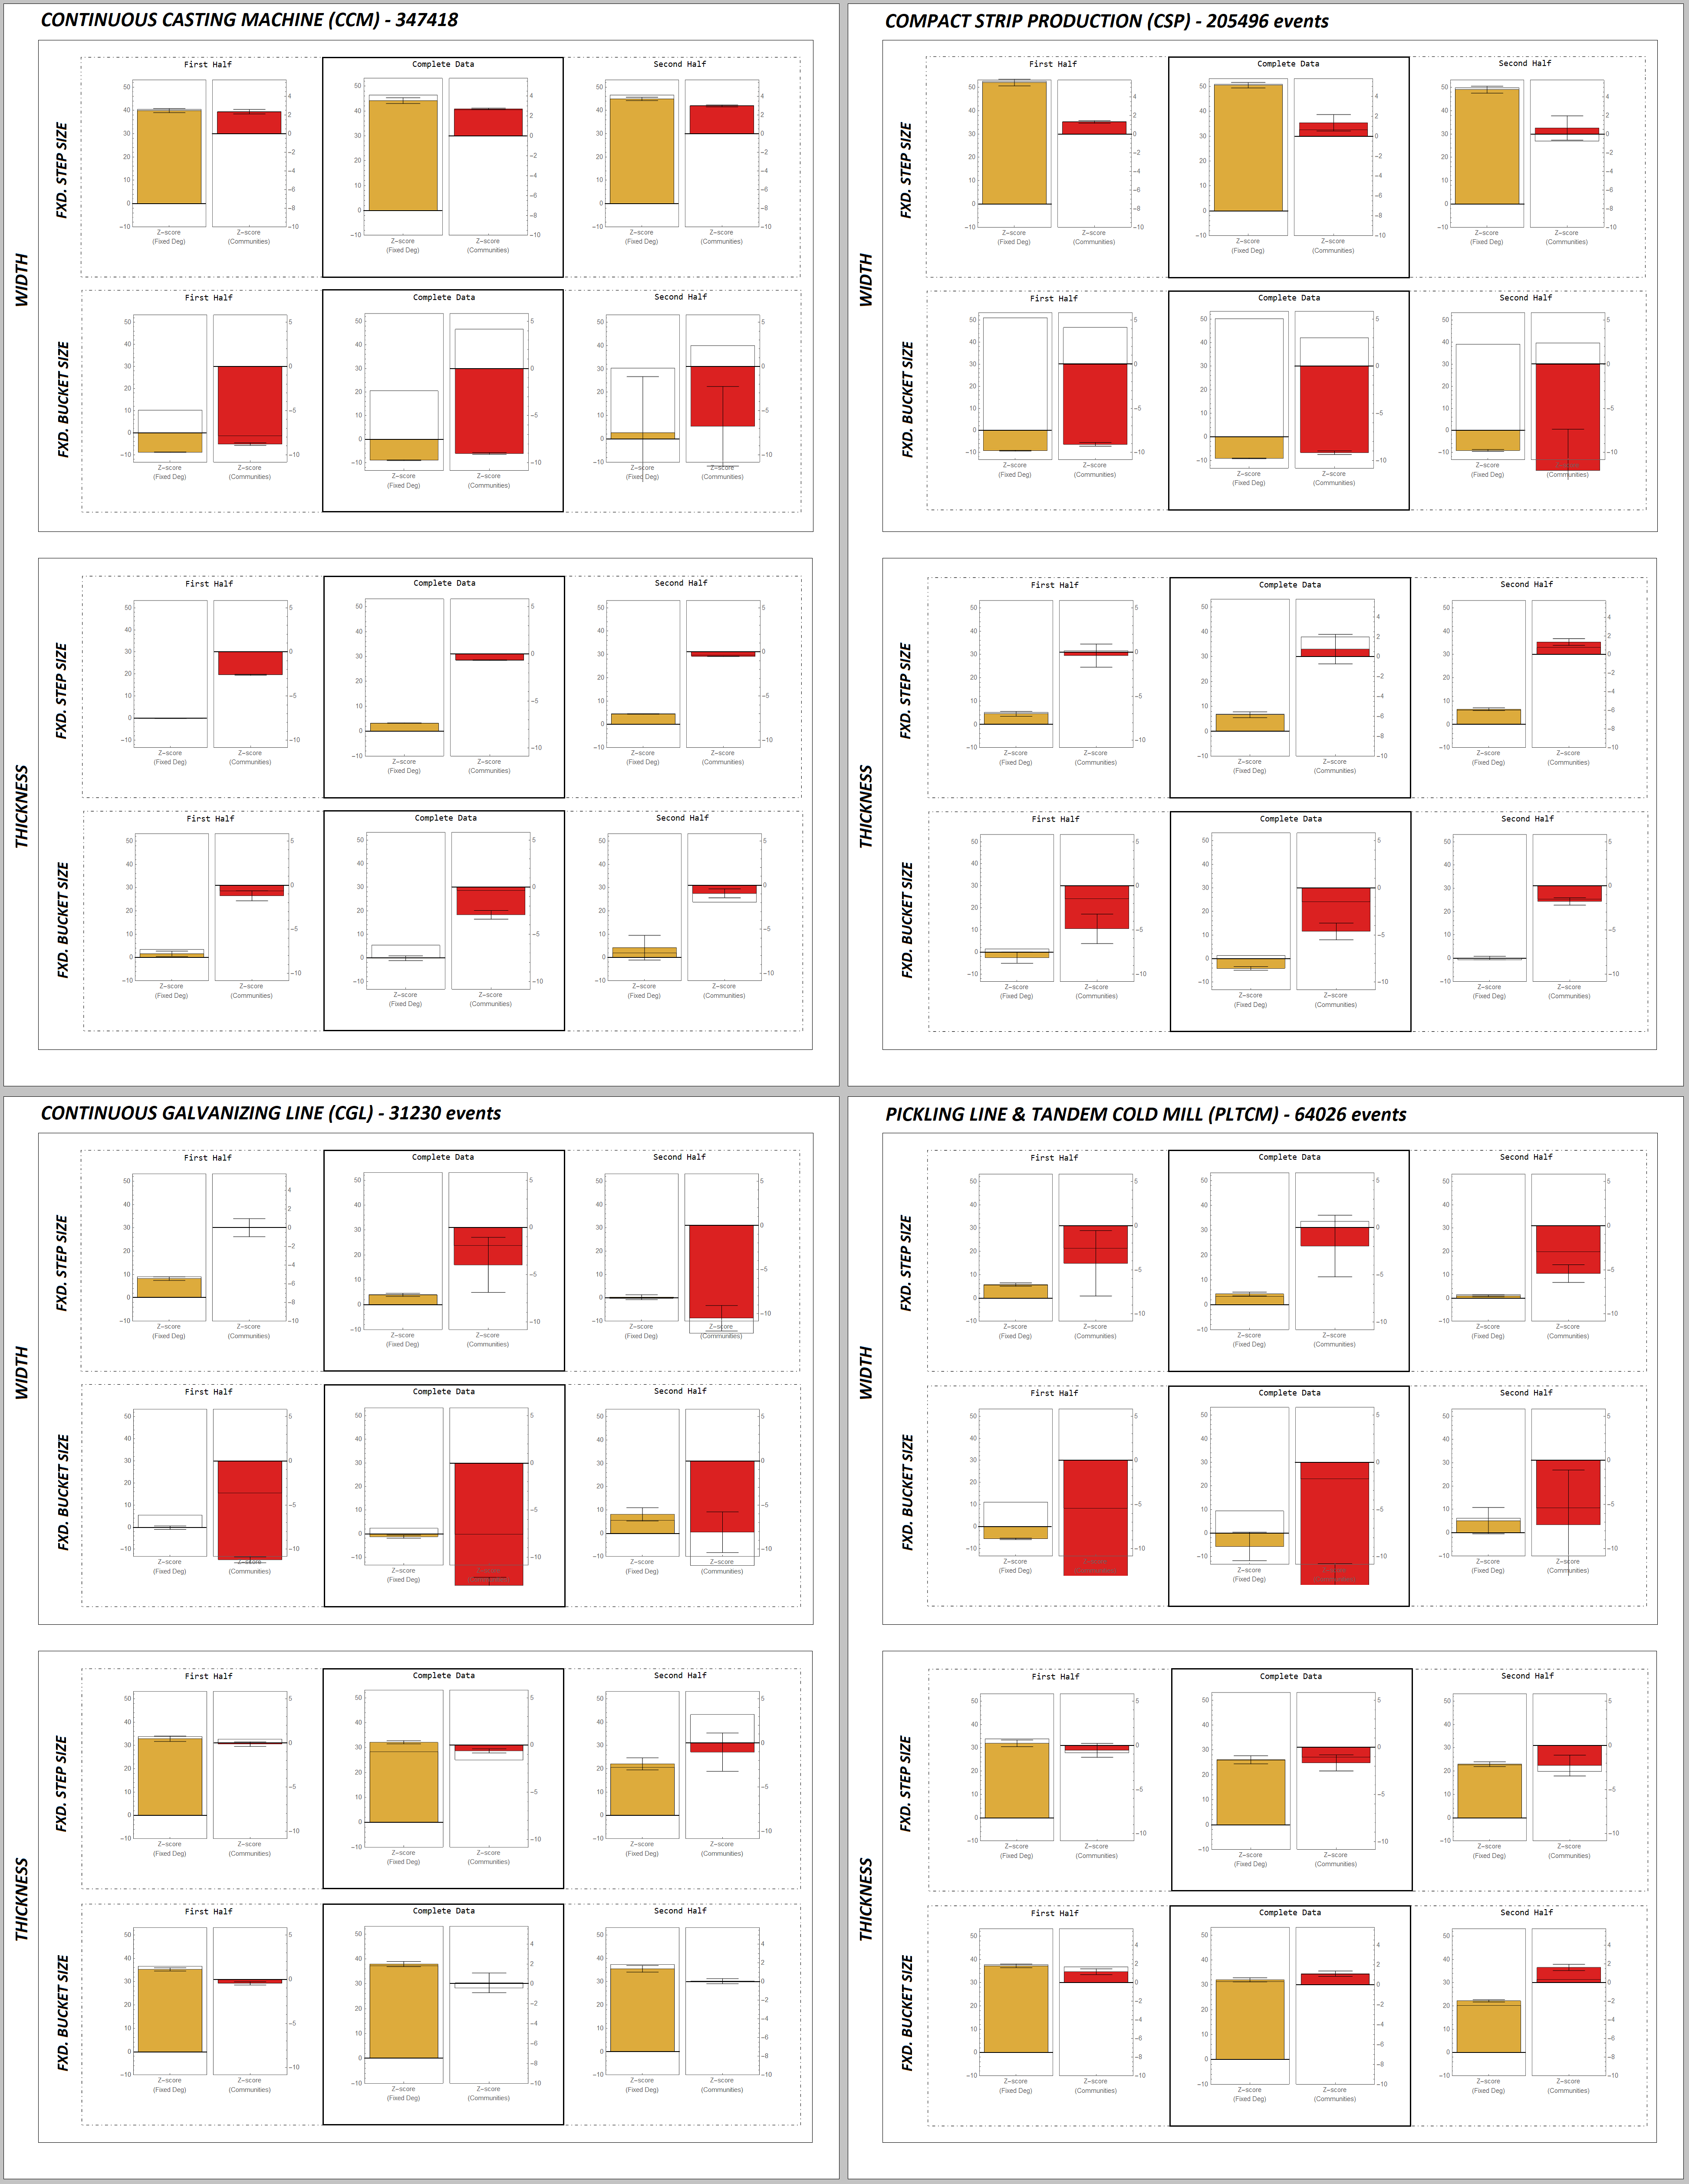
\includegraphics[width=1.05\linewidth]{../images/results-real_life_events_analysis-results.png}}
		\caption{CCM, CSP, PLTCM, CGL \aa{} Z-scores.}
		\label{figure-real-life-events-analysis-results}
	\end{center}
\end{figure}

\newcommand{\bb}{Modularity Values and Z-scores in Different Network Resolutions}
\newcommand{\cc}{Analysis Curve Plot Results:}
\newcommand{\dd}{Modularity Values and Z-scores in Sliding-time Windows\& Different Network Resolutions}
\newcommand{\ee}{Modularity Values and Z-scores in Discrete-time Windows}

FSS networks for the width feature in CCM and CSP are always modular and hierarchically organised mainly. On the other hand, FBS networks of the same feature have complicated and distorted/skewed-modular structures after checking the robustness. Until perturbing the data, the networks are modular and hierarchical, showing the unstable case of the FBS networks for the width feature in CCM and CSP.

For PLTCM and CGL, FSS and FBS networks for the thickness feature are modular and do not comprise any complex textures; therefore, that case is more reliable. FSS and FBS networks are getting complicated and distorted for the width feature, considering NM-m z-scores less than $-2$ and error bars with long T-shaped symbols.

As a summary of the bar charts in Fig.~\ref{figure-real-life-events-analysis-results}, the modular structure of the networks shifts from width to thickness when moving the observation angle from CCM and CSP to PLTCM and CGL. {\color{red}Two different binning schemes: technological constraints and load constraints, show different results through production lines going from a more general production portfolio to a more specific product portfolio}. Moreover, thickness is a more specialised feature than the width feature since the FSS and FBS networks have more significant z-scores for the thickness feature as the specialisation increases. {\color{red}Load constraint networks} do not show a significant change in width feature as going further in the production specialisation; however, {\color{red}technological constraint networks} get closer to randomness and start to get distorted in that direction.
\clearpage

\section{Simulation Events}
\subsection*{Analysis Steps and Results}
\addcontentsline{toc}{subsection}{Analysis Steps and Results}%

{\color{red} 
	
	Briefly explain \emph{in silico analyses} attempts /numerical experiments from the generated data.
	
	Plots in Part-1 of the file belong to association networks of four different synthetically created sequence data sets, and each represented in various colours: green, blue, orange, and red. Part-1 data sets were derived with fixed reaction bounds but with varying coefficients of objective functions. Part-2 also presents plots for four different synthetically created sequence data sets with fixed objective function coefficients but with variable reaction bounds.
	
	Each data set has a length of 10,000 events shared equally in 200 sequences. Randomly picked subsets of fluxes were kept the same within the sequences but having varying coefficients of objective functions.
	
		
	Limitations on resources were performed in two different ways; first, restriction on upper \& lower bounds and second, deletion of fluxes.
	
	The fluxes used in the intermediate reactions were given the range of bounds as $(-500, 500)$ since it is impossible to define infinity values in the optimisation algorithm. Randomly chosen $105$ fluxes out of $1008$ were matched with $(-5, 5)$ as the first step. Furthermore, $105$ was doubled ($212$) and then quadrupled ($425$). An important detail is that all three sets of choices were done randomly, and they are not added on top of already selected $105$. The same three sets of fluxes were used in the computations as restricted bounds in every further step.
	
	Deletion goes in the line: $0, 50, 100, 150, 200, 250, 300, 350, 400, 450$. As explained previously, deletion was done by assigning $(0, 0)$ bounds to the fluxes. On the last step, almost half of the total fluxes ($1008$) were erased.
	
	In an ideal scenario, we would find that association networks derived from the generated data, in the one case; produce high modularity for FBS and in the other case produce high modularity for FSS. Because then we have linked these two data processing schemes to different forms/to different categories of constraints.
	
	We see here that when I vary one constraint about the richness curve plots, I go from a factory that produces anything at random to a more specific factory in their production plans. The modularity at FBS increases, modularity at FSS does not increase. From left to right, I increase the constraint that the production plan (or portfolio of the factory) impose on the whole production process. The production portfolio is grouped into speciality products on the right end. An increase in modularity is only valid for the green and orange curves, which means that this effect of the changing of the portfolio only takes place. In addition, I impose certain constraints on the material flow (FBS). I enforce the production plans. In some sense, with the coefficients of objective function being symmetric around zero, I allow them also to near zero. I allow for the case this product doesn't take place. The red and the blue curves are less interesting, and they are rather serving as an orientation. We wouldn't expect them to be severely affected by changes in the richness of the objective function because the terms are cancelled out. So the interesting curves are the green and orange one that we can argue for it. We don't expect a strong impact of the richness of the objective functions for these cases (red and blue), and that's indeed what I numerically observed. So it makes sense to have these curves, but the interesting curves are the green and the orange ones.
	Blue curve z-score is very hard to compute, and we should not trust it that much; also, its z-score curve is lower than the red z-score curve. 
}

 \begin{figure}[!ht]
	\begin{center}
		\makebox[\textwidth]{
			\centering
			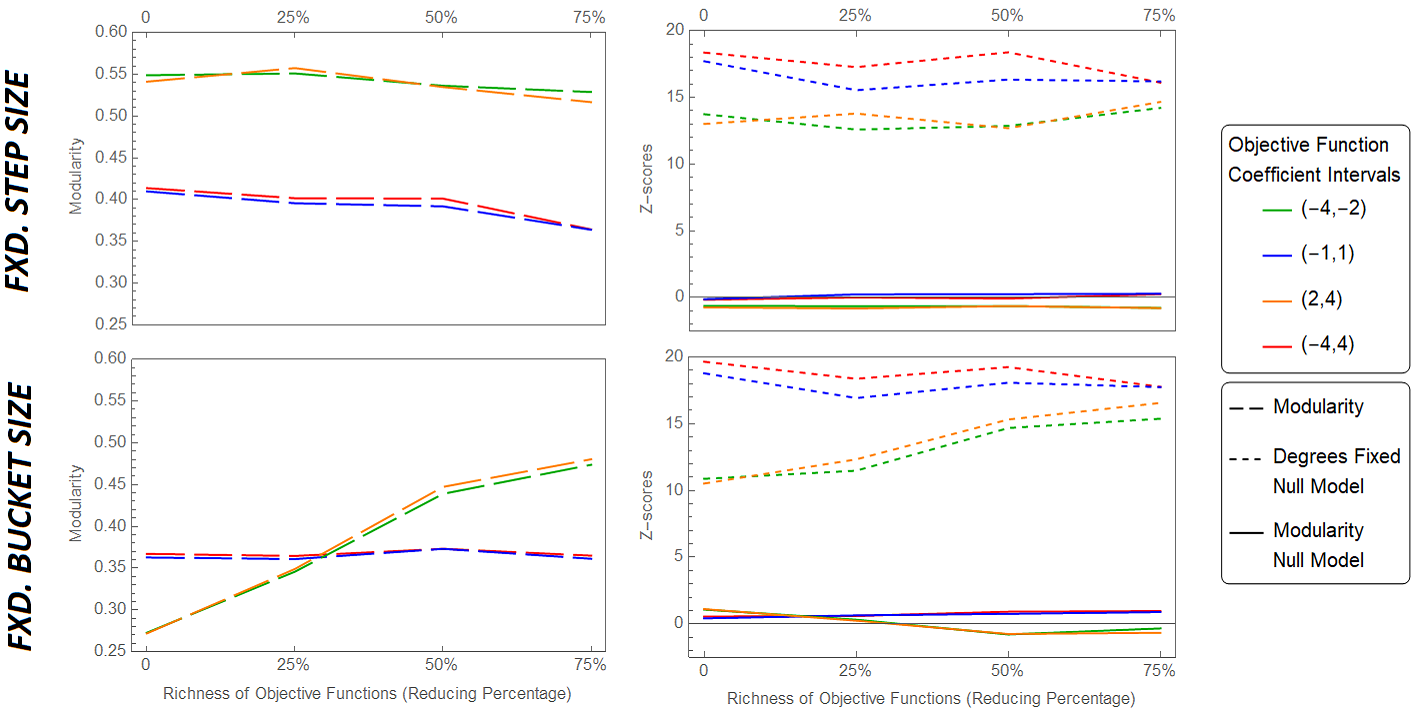
\includegraphics[width=1.03\linewidth]{../images/results-simulation-results.png}}
		\caption{Simulation Analysis Curve Plot Results: Modularity Values and Z-scores.}
		\label{figure-FBA-results}
	\end{center}
\end{figure}

%\begin{equation} %\tag{8}
%	(O.V)_{1}= (o_{1,1}v_{1} + o_{1,2}v_{2} + \dots + o_{1,r}v_{r})
%\end{equation}

%\begin{equation} %\tag{8}
%	(O.V)_{2}= (o_{2,1}v_{1} + o_{2,2}v_{2} + \dots + o_{2,r}v_{r})
%\end{equation}

%\begin{equation} 	
%	(O.V)_{50}= (o_{50,1}v_{1} + o_{50,2}v_{2} + \dots + o_{50,r}v_{r})
%\end{equation}

%\begin{equation} 	
%	(O.V)_{51}= (o_{1,1}v_{1} + o_{1,2}v_{2} + \dots + o_{1,r}v_{r})
%\end{equation}

%\begin{equation} 	
%	(O.V)_{100}= (o_{50,1}v_{1} + o_{50,2}v_{2} + \dots + o_{50,r}v_{r})
%\end{equation}

%\begin{equation} 	
%	(O.V)_{10000}= (o_{50,1}v_{1} + o_{50,2}v_{2} + \dots + o_{50,r}v_{r})
%\end{equation}

%\begin{table}[hb!]
%	\centering
%	\begin{tabular}{|cccccc|l}
%		\cline{1-6}
%		\makecell{Event\\ID} && \makecell{Bio\\Mass} 	&& \makecell{Seq.\\ID} &  \\ \cline{1-6}
%		1 	      && $m_{1}$  	&& 1 		   	&  \\
%		2 		  && $m_{2}$	&& 1 		   	&  \\
%		3 	      && $m_{3}$	&& 2 		    &  \\
%		\vdots	  && \vdots && \vdots 	    &  \\
%		n 		  && $m_{n}$	&& k 		    &  \\ \cline{1-6}
%	\end{tabular}
%	\caption{Arbitrarily Created Data Set $D$.}
%	\label{Tab:D-dataset}
%\end{table}